\documentclass[border=2pt,svgnames,tikz]{standalone}
\usepackage{fontspec}
\setmainfont{Source Serif 4}
\setsansfont{Source Sans 3}
\setmonofont{Source Code Pro}
\usepackage{ctex}
\setCJKmainfont[BoldFont=Source Han Sans CN]{Source Han Serif CN}
\usetikzlibrary{arrows.meta, patterns, positioning, calc}

\begin{document}
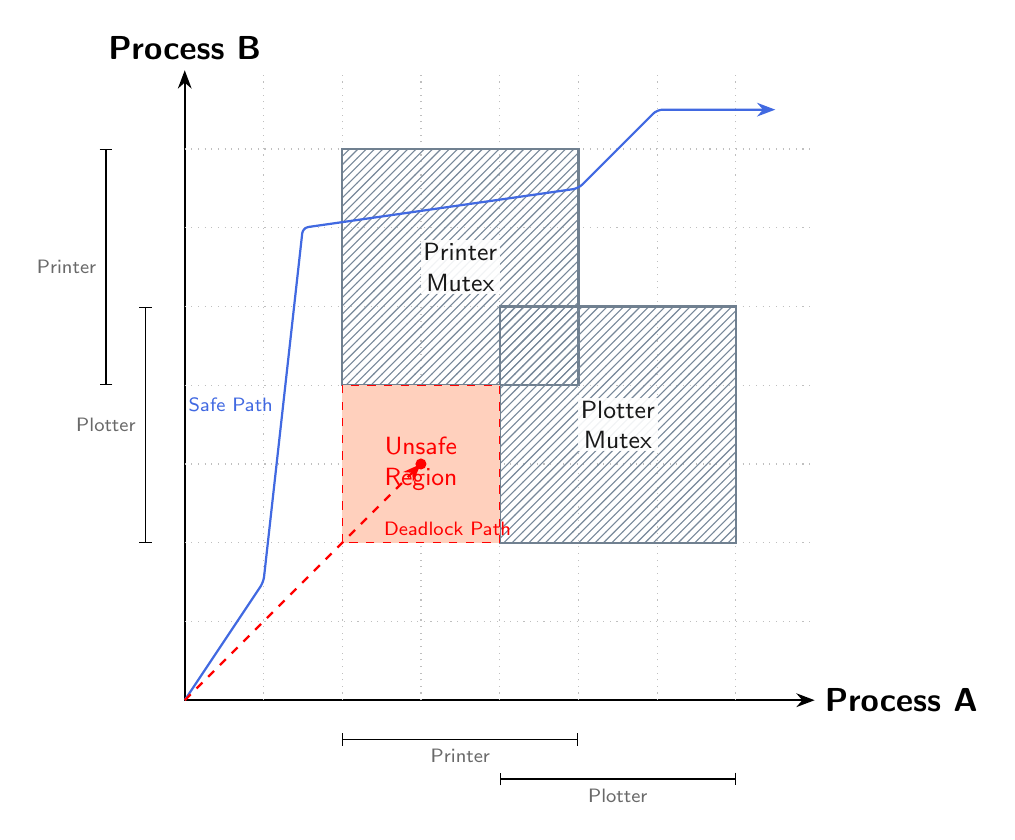
\begin{tikzpicture}[
    >=Stealth,
    axis/.style={->, thick, line cap=rect},
    process_label/.style={font=\sffamily\large\bfseries},
    resource_label/.style={font=\scriptsize\sffamily, color=DimGray},
    mutex_region/.style={pattern=north east lines, pattern color=LightSlateGray, draw=SlateGray, thick},
    unsafe_region/.style={fill=LightSalmon!50, draw=Red, dashed},
    trajectory/.style={thick, RoyalBlue, ->, rounded corners=2pt},
    grid_line/.style={dotted, Gray!50}
]

% Coordinates
\def\MaxX{8}
\def\MaxY{8}

% Process A (X-axis) Resource Usage
% Printer: 2 to 5
% Plotter: 4 to 7
\def\APrinterStart{2}
\def\APrinterEnd{5}
\def\APlotterStart{4}
\def\APlotterEnd{7}

% Process B (Y-axis) Resource Usage
% Plotter: 2 to 5
% Printer: 4 to 7
\def\BPlotterStart{2}
\def\BPlotterEnd{5}
\def\BPrinterStart{4}
\def\BPrinterEnd{7}

% Unsafe Region Calculation
% A holds Printer (2-5), needs Plotter (starts at 4)
% B holds Plotter (2-5), needs Printer (starts at 4)
% Intersection of "A holds Printer" and "B holds Plotter" is [2, 4] x [2, 4]
% Wait, A holds Printer until 5. B holds Plotter until 5.
% But A requests Plotter at 4. B requests Printer at 4.
% So the deadlock happens if they both reach the request point.
% The unsafe region is the area from which you inevitably hit the deadlock.
% It is the rectangle defined by:
% X range: [APrinterStart, APlotterStart] -> [2, 4]
% Y range: [BPlotterStart, BPrinterStart] -> [2, 4]
% Actually, once you are in [2,4]x[2,4], you can't go past x=4 (blocked by Plotter Mutex) or y=4 (blocked by Printer Mutex).
% So [2,4]x[2,4] is the unsafe region.

% Axes
\draw[axis] (0,0) -- (\MaxX,0) node[right, process_label] {Process A};
\draw[axis] (0,0) -- (0,\MaxY) node[above, process_label] {Process B};

% Grid and Ticks (Optional, but helps reading)
\foreach \x in {1,...,7} \draw[grid_line] (\x,0) -- (\x,\MaxY);
\foreach \y in {1,...,7} \draw[grid_line] (0,\y) -- (\MaxX,\y);

% Mutex Regions (Impossible States)
% Printer Mutex: A has Printer (2-5) AND B has Printer (4-7)
% Overlap: x in [2,5], y in [4,7]
\filldraw[mutex_region] (\APrinterStart, \BPrinterStart) rectangle (\APrinterEnd, \BPrinterEnd);
\node[font=\small\sffamily, align=center, fill=white, inner sep=1pt, opacity=0.9] at ({(\APrinterStart+\APrinterEnd)/2}, {(\BPrinterStart+\BPrinterEnd)/2}) {Printer\\Mutex};

% Plotter Mutex: A has Plotter (4-7) AND B has Plotter (2-5)
% Overlap: x in [4,7], y in [2,5]
\filldraw[mutex_region] (\APlotterStart, \BPlotterStart) rectangle (\APlotterEnd, \BPlotterEnd);
\node[font=\small\sffamily, align=center, fill=white, inner sep=1pt, opacity=0.9] at ({(\APlotterStart+\APlotterEnd)/2}, {(\BPlotterStart+\BPlotterEnd)/2}) {Plotter\\Mutex};

% Unsafe Region
\filldraw[unsafe_region] (\APrinterStart, \BPlotterStart) rectangle (\APlotterStart, \BPrinterStart);
\node[font=\small\sffamily, text=Red, align=center] at ({(\APrinterStart+\APlotterStart)/2}, {(\BPlotterStart+\BPrinterStart)/2}) {Unsafe\\Region};

% Axis Labels for Resources
% Process A
\draw[|-|] (\APrinterStart, -0.5) -- node[below, resource_label] {Printer} (\APrinterEnd, -0.5);
\draw[|-|] (\APlotterStart, -1.0) -- node[below, resource_label] {Plotter} (\APlotterEnd, -1.0);

% Process B
\draw[|-|] (-0.5, \BPlotterStart) -- node[left, resource_label] {Plotter} (-0.5, \BPlotterEnd);
\draw[|-|] (-1.0, \BPrinterStart) -- node[left, resource_label] {Printer} (-1.0, \BPrinterEnd);

% Trajectories
% 1. Safe Trajectory
\draw[trajectory] (0,0) -- (1, 1.5) -- (1.5, 6) node[pos=0.5, left, font=\scriptsize\sffamily, text=RoyalBlue] {Safe Path} -- (5, 6.5) -- (6, 7.5) -- (7.5, 7.5);

% 2. Deadlock Trajectory (entering unsafe region)
\draw[trajectory, Red, dashed] (0,0) -- (3, 3) node[pos=0.8, below right, font=\scriptsize\sffamily, text=Red] {Deadlock Path};
\fill[Red] (3,3) circle (2pt);

\end{tikzpicture}
\end{document}
